
\section{Implementation Details}
\subsection{High-Level Overview and Design}
We will provide two configurations that this service can be deployed as: a simple single single system deployment and a more complex highly available deployment that uses a reverse proxy to load balance between the applications. All version will consist of at least the main \textit{Probably Secure Password Manager} server running on Node JS as a docker container, and a MongoDB docker container that is accessable to the \textit{Probably Secure Password Manager} server.

\begin{figure}[h]
  \centering
  \begin{subfigure}{0.45\textwidth}
    \centering
    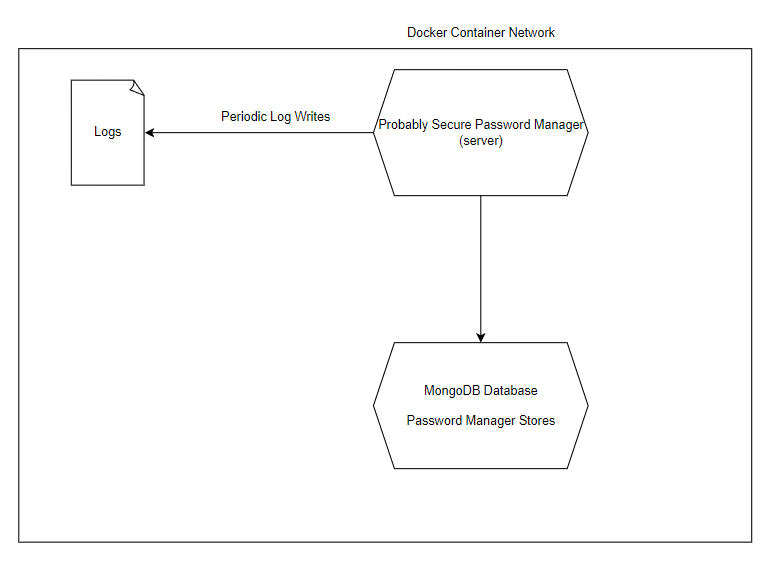
\includegraphics[width=\textwidth]{Single.png}
    \caption{Single Server}
  \end{subfigure}
  \hfill
  \begin{subfigure}{0.45\textwidth}
    \centering
    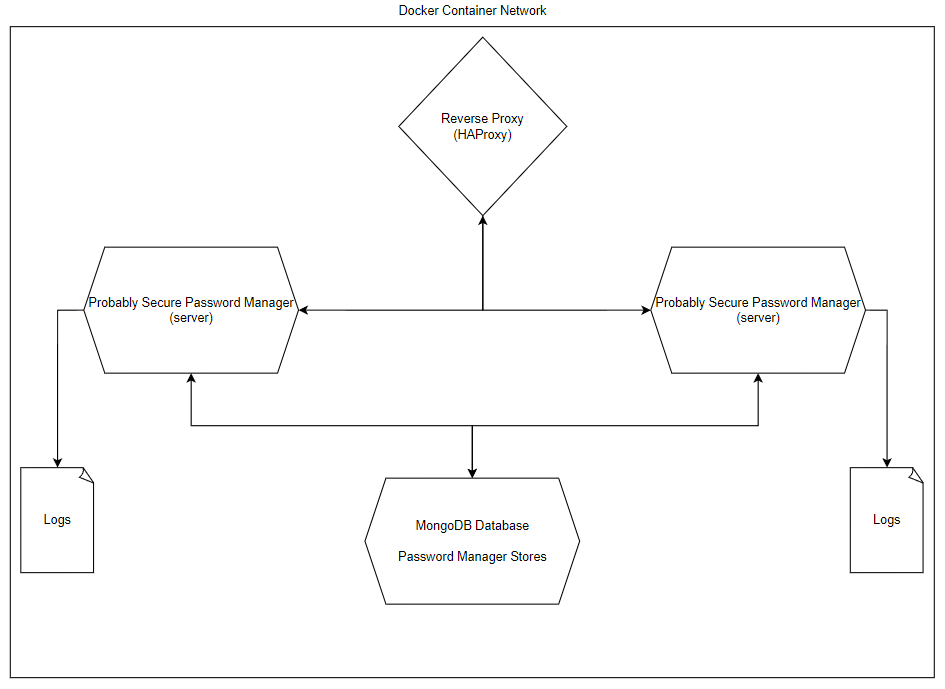
\includegraphics[width=\textwidth]{HA.png}
    \caption{High Availability}
  \end{subfigure}
  \caption{Server Deployments}
\end{figure}



\subsection{Overview of Components and Modules}

\begin{tabular}{|c|p{6cm}|c|}
    \hline
    \textbf{Component/Module}& \textbf{Purpose} & \textbf{Language}\\
    \hline
    Authentication Component (Server) & Handle the Authentication of Users and API Requests. & JS (Express)\\ 
    \hline
    Logging Component (Server) & Manage logging levels and messages. & JS (Express)\\
    \hline
    User Management (Server) & Add, and remove users. Change Passwords. & JS (Express)\\
    \hline
    User Dashboards (Server) & Populate pages with a user's stored passwords. & JS (Express)\\
    \hline
    Vulnerability Management (Server) & Configure and view vulnerability status. & JS (Express)\\
    \hline
    User Interface (FE) & Reactive User Frontend. & JS (React)\\
    \hline
    Database & Store user access credentials and saved data. & External (MongoDB)\\
    \hline
\end{tabular}

\subsection{Overview of 3rd Party Components and Modules}

\begin{tabular}{|c|c|c|}
    \hline
    \textbf{Component/Module}& \textbf{Use Case}&\textbf{Licence}\\% &\textbf{URL}\\

    \hline
    MongoDB & Primary Database & \href{https://www.mongodb.com/legal/licensing/server-side-public-license}{Server Side Public Licence}\\ 
    \hline
    Passport & User Authentication Framework & \href{https://github.com/jaredhanson/passport/blob/master/LICENSE}{MIT}\\ 
    \hline
    Express JS & Backend Framework & \href{https://github.com/expressjs/express/blob/master/LICENSE}{MIT}\\ 
    \hline
    React JS & Frontend JS Framework & \href{https://github.com/facebook/react/blob/main/LICENSE}{MIT}\\
    \hline
    cors & Middlewear & \href{https://www.npmjs.com/package/cors}{MIT}\\
    \hline
    dotenv & Environment Variable Management & \href{https://github.com/motdotla/dotenv/blob/master/LICENSE}{BSD 2-Clause}\\
    \hline
    Docker Engine & Containerization Platform & \href{https://github.com/moby/moby/blob/master/LICENSE}{Apache License, Version 2.0}\\ 
    \hline
    Piano & Logging Library & \href{https://github.com/pinojs/pino/blob/main/LICENSE}{MIT}\\
    \hline
\end{tabular}\\\\
% \subsection{Overview of 3rd Party Services and APIs}
\textbf{As of the time of writing, there are no plans to use thrid party services or APIs.}

\subsection{Overview of REST Endpoints}

\textbf{/api/admin}: Utilized by the administrator to access user information, and manage users on the server. Contains action to do, authorization token, and the action information.\\
\textbf{/api/auth}: Authenticate to the server and gain access tokens. Contains user to authenticate as and their password.\\
\textbf{/api/internal}: Provides internal management information. Contains target data and an authorization token.\\
\textbf{/api/vulns}: Utilized by the administrator to toggle vulnerabilities on the server. It contains target vulnerability, authorization token, and if that should be enabled or disabled.\\
\textbf{/api/alogs}: Request a subset of the most recent logs. It contains an authorization token.\\
\textbf{/api/tlogs}: Configure logging capabilities of the server. Contains authorization token and the log level.\\
\textbf{/api/passwd}: Store, or access a password the server currently manages. Contains the user's authentication token and the body to store the user's password\\
\textbf{/api/share}: Used to share a password with a given user. Contains the user's authentication token, the password ID to share and the target user.